%%%%%%%%%%%%%%%%%%%%%%%%%%%%%%%%%%%%%%%%
%   Original by                                   %
% Athanassios Protopapas, October 2005 %
% Mini-example for using apa.cls       %
%                                      %
% modified by William Revelle, August, 2007 
%%%%%%%%%%%%%%%%%%%%%%%%%%%%%%%%%%%%%%%%

\documentclass[doc]{apa}%can be jou (for journal), man (manuscript) or doc (document)
%
%
%these next packages extend the apa class to allow for including statistical and graphic commands
\usepackage{url}   %this allows us to cite URLs in the text
\usepackage{graphicx}  %allows for graphic to float when doing jou or doc style
\usepackage{amssymb}  %use formatting tools  for math symbols
% type setting of functions, packages, and R follows a particular style
\let\proglang=\textsf
\newcommand{\R}{\proglang{R}}
\newcommand{\pkg}[1]{{\normalfont\fontseries{b}\selectfont #1}}
\newcommand{\Rfunction}[1]{{\texttt{#1}}} 
\newcommand{\fun}[1]{{\texttt{#1}}} 
\newcommand{\Robject}[1]{{\texttt{#1}}} 
%
%
%Here is where we start the important APA stuff

\usepackage{verbatim}
\usepackage{pseudocode}
\usepackage{algorithm}
%\usepackage{algorithmic}
\usepackage{amsmath}
\usepackage{amsthm}
\usepackage{algpseudocode}
\usepackage{algorithmicx}% http://ctan.org/pkg/algorithmicx

% ================ ALGORITHM ENVIRONMENT ================
\newcounter{numberedAlg}% Algorithm counter
\newenvironment{numberedAlg}[1][]%
  {% \begin{numberedAlg}[#1]
    \needspace{2\baselineskip}% At least 2\baselineskip required, otherwise break
    \noindent \rule{\linewidth}{1pt} \endgraf% Top rule
    \refstepcounter{numberedAlg}% For correct reference of algorithm
    \centering \textsc{Algorithm}~\thenumberedAlg%
    \ifthenelse{\isempty{#1}}{}{:\ #1}% Typeset name (if provided)
  }{% \end{numberedAlg}
  \noindent \rule{\linewidth}{1pt}% Bottom rule
  }%

\title{Engineering Networks for Optimal Robustness}
\author{Christopher A. Wood}
\affiliation{Department of Computer Science \\ Rochester Institute of Technology}

\abstract{Military and civillian network-oriented operations have seen very high growth rates in recent years. Along with this expansion has been the advancement of sophisticated network attacks against such networks and increased probability of network failure. In order to handle such failures, networks must be designed to be robust to these attacks. Thus, both the physical characteristics (i.e. the channel bandwidth and transmission media) and the topological properties of a network have a large impact on the measure of robustness of networks to such events. 

In this paper we present research findings that attempt to measure network robustness, optimize existing network topologies to attain maximal robustness, and even construct arbitrary networks to exhibit high resistance to network failures. In doing so, we also discuss some of the common sources of topology changes in a network that stimulated this research, such as targeted and random network failures. We then conclude with observations about the current state-of-the-art in network stuctures and their relationship with network robustness, which serve as heurstic guidelines for network engineers when designing such systems.}

\shorttitle{Engineering Networks for Optimal Robustness}
\rightheader{Engineering Networks for Optimal Robustness}
\leftheader{Christopher A. Wood}

\begin{document}
\maketitle   

\section{Introduction}

Military and civilian communications have seen two common trends in rencent years: an increase in network-oriented operations and an increase in high-risk malicious attacks against networks that facilitate such operations \cite{Bernardnetworkrobustness}. It is vital that the underlying network infrastructure for such operations can defend against such emerging attacks that focus on specific nodes or links in the network or random failures that occur throughout. This requirement has stimulated research in two separate directions: the stability of communication protocols to handle such attacks and failures, as well as the topological analysis of the network's resilience to such attacks. The measure of resilience to such attacks or failures is referred to as the robustness of a network, and is a topic that has been studied analytically and experimentally extensively in recent years.

The physical properties of networks, such as the channel bandwidth and transmission media, have a significant effect on the measure of robustness of a network due to the constraints they place on traffic routing changes in the event of network failures. Similarly, the communication and routing protocols that are utilized to handle the traffic flow also effect the traffic load for individual nodes and links when network failures occurs, which in turn effects the network robustness. However, recent research efforts have approached the study of network robustness from the topological domain. Such an analysis calls on methods from graph theory, statistics, and probability theory in order to solve more general questions about the relationship between the structure of a graph and its robustness.

In this paper we survey research that has been centered around the theoretical analysis of network topology and its impact on the measure of robustness. In doing so, we also discuss some common sources of topology changes in networks (i.e. targeted attack models and failures), techniques to measure the robustness of a network, and methods that have been utilized to study and optimize network robustness for random networks with arbitrary structural characteristics.

\section{Fundamentals and Notation}
\label{Definitions}

It is natural to model a communication network as a weighted undirected graph $G = (V,E)$, where $V$ is a set of nodes (or vertices) and $E$ is a set of edges (or links) that represent physical connections between such vertices. We also assign weights $w \in \mathbb{R}$ for each edge, where unweighted edges receive a weight of $0$. For convenience, we let $N = |V|$ and $M = |E|$. The topology of a network can thus be visualized graphically using elements from these two sets. 

In order to discuss the measures of network robustness and analytical techniques used to study the network robustness in the topological domain, it is necessary to introduce the following definitions. \\

\textbf{Definition 1:}
The \textbf{degree} of a vertex $u \in V$ for any graph $G = (V,E)$ is said to be the total number of edges incidenct to $u$. In other words, $deg(u) = \sum_{(u,v) \in E} 1$ for all $v \in V$. We denote the minimum degree over all vertices in a graph $G$ as $\delta(G)$. In network analysis it is common to utilize the degree distribution of a graph as the basis for many measurements. As such, we denote $k$ as the average degree distribution for a graph $G$.\\

%Component
\textbf{Definition 2:}
A \textbf{component} of a graph $G = (V,E)$ is a subgraph $G' = (V',E')$ in which there exists a path between all vertices $u, v \in V'$. Further, a graph $G$ is said to be \textbf{connected} if and only if there is at most $1$ conneted component in $G$ (i.e. the entire graph). If a graph is not connected, then it is \textbf{disconnected}.\\

% vertex and edge connectivity
\textbf{Definition 3:}
The \textbf{vertex connectivity} of a graph $G = (V,E)$, denoted $\kappa(G)$, is defined as the minimum number of nodes whose deletion will leave the graph disconnected. Similarly, the \textbf{edge connectivity} of a graph $G$, denoted $\lambda(G)$, is defined as the minimum number of edges whose deletion will leave the graph disconnected.\\

\textbf{Definition 4:}
The \textbf{distance} between any two vertices $u, v \in V$ in a graph $G = (V,E)$ is defined as the sum of the link weights along the edges that correspond to the shortest path between $u$ and $v$.

\section{Network Performance}
\label{NetworkFunctionality}

In general, high performance networks exhibit high throughput and low latency between nodes in the same network. Other quality metrics include the number of hops between nodes, distance between two nodes, jitter on the transmission medium, channel loss rate, and the channel bandwidth (or capacity) \cite{LargeNetworkRobustnessPVM}. These measurements are often used to assign weights to the links in a network in order to analytically determine the optimal network designs. In particular, the weight of links are usually expressed as a linear combination of such quality metrics that can be modified to reflect the real-world nature of the networks. However, when considering only the topology of a network, it is common to assign uniform weights of $1$ to all link edges. By doing so, we need only consider the topology of the network when quantifying its performance. 

Perhaps the most natural topology-based measurement for performance is the average geodesic path length between any two nodes in a network. This measurement equates to the average shortest path) and vertex and edge betweeness (which are essentially measures of centralities located within a graph). Mathematically, the average geodesic length $L$ can be defined as follows:
\begin{eqnarray}
L(d(v,w)) = \frac{1}{N(N-1)}\sum_{v \in V(G)}\sum_{w \not= v \in V(G)} d(v,w),
\end{eqnarray}
where $d(v,w)$ is the distance of the shortest path between vertices $v$ and $w$, and $N(N-1)$ is the total number of pairs of vertices, independent of whether or not each pair represents an edge in $E(G)$. The most immediate result from this measurement is that large values for $L$ indicate that the average length between any two nodes in the network is long, and thus the latency between two nodes will be proportionally large as well. 

Another important metric that measures the functionality of a network is the measure of vertex and edge centrality in the network. A high measure of centrality may indicate more traffic funnels through a vertex or an edge, which means that there may be more backup nodes available in the event that this node or link fails. High measures of centrality also imply that any attacks on the associated vertex or edge would most likely have an negative impact on the traffic in the network by increasing the load on neighboring nodes and increasing the average geodesic path length. 

Although there is not a single definition for this metric, Holme et al \cite{Attacks} propose the use of the following definitions for vertex $C_{B}(v)$ and edge $C_{B}(e)$ centrality.
\begin{eqnarray}
C_{B}(v) = \sum_{w \not= x \in V(G)} \frac{\sigma_{wx}(v)}{\sigma_{wx}},
\end{eqnarray}
\begin{eqnarray}
C_{B}(e) = \sum_{w \not= x \in V(G)} \frac{\sigma_{wx}(e)}{\sigma_{wx}}
\end{eqnarray}
In these equations, $\sigma_{wx}(v)$ is the number of paths between $w$ and $x$ that pass through $v$ and $\sigma_{wx}$ is total of paths from $w$ to $x$ (notice that $\sigma_{wx}(v) \leq \sigma_{wx}$), and $\sigma_{wx}(e)$ is the number of paths between $w$ and $x$ that contain $e$ and $\sigma_{wx}$ is total of paths from $w$ to $x$ (notice again that $\sigma_{wx}(e) \leq \sigma_{wx}$).

It is important to note that the centrality of a vertex and an edge are not the same metrics \cite{Attacks}. Also, it is clear that a robust network will have an overall high level of vertex or edge centrality, as this indicates that there are more backup nodes or links available to use in the event of a network failure.

%\section{Network Attacks}
%HDA - high degree adaptiveness - onion
% from: http://polymer.bu.edu/~hes/networks/hsmah11.pdf

%more from http://www.ncbi.nlm.nih.gov/pubmed/12059649
%Some other attacks are described in \cite{Attacks}

\section{Attack Models}
\label{AttackStrategies}

\subsection{Targeted Attacks}
Attacks on large scale networks are not usually ad-hoc; they are based on a logical and structured strategy for dereasing the connectivity of the network by removing select nodes or links from the network in as few steps as possible. Clearly, deleting all nodes from a network would yield the maximum decrease in connectivity. However, such attacks are not practical, so these strategies must be considered at a smaller scale. 

Most practical attacks are focused on the objective of decreasing the number of total links in the network or the average geodesic length (or both). Consider, for example, the situations of cutting communication cables or performing a DDOS attack on a node or server with a high measure of centrality. Such attacks would decrease the number of edges in the network graph and increase the average geodesic path length, respectively, which both result in decreased performance by some factor.

From the definitions presented earlier, we can see that the number of edges in the network is directly related to the degree of each vertex (in fact, we know that $2|E(G)| =\sum_{v \in V(G)}deg(v)$). On the other hand, the measure of centrality of a vertex or edge is more related to the average geodesic path length in the network. As such, we consider practical attack patterns that focus on decreasing both of these measurements by targeting individual vertices and/or edges, as well as randomized attacks that have no specific targets. 

In general, most targeted attacks fall under one of the following four categories: (1) \emph{ID removal}, or initial degree distribution vertex or edge removal, (2) \emph{IB removal}, or initial betweenness distribution vertex or edge removal, (3) \emph{RD removal}, or recalculated degree distribution vertex or edge removal, and (4) \emph{RB removal}, recalculated betweenness distribution vertex or edge removal. An example of initial and recalculated edge-centric attacks on a fixed graph topology is shown in Figure 1 \cite{Attacks}.

\begin{figure}[h!]
	\label{fig:attackPics}
	\centering
		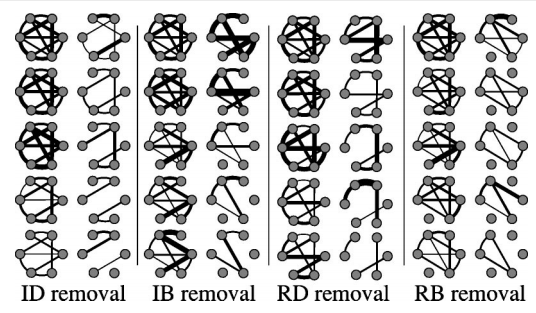
\includegraphics[width=0.5\textwidth]{edge_attacks.png}
	\caption{Various edge-centric attacks for a fixed graph topology.}
\end{figure}

RD and RB attacks on vertices yield the optimal results because they take a greedy approach to decrease the target metric. However, the implication of these attacks is that there exists an efficient and tractable way to measure these metrics after every change, which isn't always the case (especially when the topology of the network is unknown). Therefore, ID and IB attacks are more realistic, but they also assume some prior knowledge of the network infrastructure before the attack begins. 

Furthermore, it should be noted that both the ID and RD attacks are computationally less taxing than IB and RB attacks \cite{Attacks}. In fact, the time complexity of a successful ID attack (and subsequently, an entire RD attack), runs in linear time with respect to N, whereas the time complexity of betweenness-based attacks has a time complexity of $O(NL)$. The implication of this is that the adversary must make tradeoffs based on their knowledge of the network infrastructure when determining which attack to conduct. This decision is further influenced by the amount of knowledge that the attacker requires for such attacks. For example, with knowledge of an entire network infrastructure it would be possible for an attacker to make globally optimal decisions for each attack. However, with only a limited view of the network, the attacker must make locally optimal decisions for each attack. 

\subsection{Random Failures}
\label{RandomFailures}
While targeted attacks model common scenarios in the real-world, it is often useful to disregard the source and victim of such attacks and generalize the problem of network failures to encompass both random node and link failures. By doing so, we assume that each node and link has a fixed probability $p$ and $q$ of failing, where the exact cause of the failure is not know and is not important. Furthermore, failures are typically seen as independent events \cite{RandomStudy}. 

Such models are useful when analyzing complex networks such as the Internet and other related military communication networks. This is primarily because it is difficult to formulate precise relationships between the network structure and its robustness under arbitrary failures when analyzing specific network topologies modified by select attacks. Generalizing the concept of network failure into probabilistic events and assuming as little information as possible about the structure of a network enables researchers to study the problem of network robustness at a very high-level, which usually yields results that can apply to most networks. 

\section{Network Robustness}
%http://arxiv.org/pdf/1203.2982v1.pdf

\subsection{Static Robustness Measurements}

Two common ways to calculate the robustness of a network are to consider the topological changes that are induced from the removal of nodes or links. Examining the robustness of a network from the perspective of individual nodes, since they are  usually the primary targets in malicious or non-malicious network attacks. Using this idea, Herrmann et al defined a concise equation for calculating the robustness based on the largest connected component $S(q)$ after $q$ hub nodes are removed from the network. Mathematically, this can be defined as follows \cite{Onion}:
%24: http://polymer.bu.edu/~hes/networks/hsmah11.pdf
\begin{eqnarray}
R_{N} = \frac{1}{N}\sum_{q=1/N}^{1}S(q)
\end{eqnarray}
This calculation has been mathematically verified to represent the exact amount of nodes that need to be deleted for the network to collapse when targeted by high-degree adaptive attacks, which are a specific class of attacks that attempt to remove highly connected nodes from the network. 

%TODO: http://arxiv.org/pdf/1203.2982v1.pdf, \cite{NRMalicious}

From the perspective of the communication links that exist in a network, the most successful attacks are those that take down the take down the most important or centralized communication links. As such, a common research trend has been to examine the largest components of a network with respect to the edge-betweenness, link clustering coefficient, and degree product \cite{NRMalicious}. One common measurement of the robustness of a network with respect to these metrics and the largest component of a network $S(p)$ after the removal of $p$ links is shown below:
\begin{eqnarray}
R_M = \frac{1}{M}\sum_{p = 1/M}^{1}S(p)
\end{eqnarray}
This measurement is mathematically similar to the previous node-based calculation, but instead of considering the density of the nodes in the entire component, it considers the density of the edges. 

Due to the typical attacks that are launched on networks, such as large-scale DDoS attacks that take both nodes and links to that node offline, it is natural to extend the concept of network robustness to consider both node and link failures simultaneously. However, rather because the two aforementioned measurements are based on two separate dimensions of networks, it is not simply a matter of merging them together to yield the optimum result. Instead, the measurement is typically abstracted into the context of the attack that is launched on a network, where the input parameter into the largest component is now the number of steps $t$ that have been completed at a given instance in time. Mathematically, this hybrid measurement $R$ can be computed as follows \cite{NRMalicious}:
\begin{eqnarray}
R_S = \frac{1}{M}\sum_{t  = 1}^{M}S(t)
\end{eqnarray}

\subsection{Dynamic Robustness Measurement}
%http://www.cs.berkeley.edu/~yaron/papers/dyner.pdf

It is also possible to measure the robustness of a network by simulating artificial node or link failures and analyzing the effect on the underlying connection graph. One recently proposed method that follows this approach is called the Dynamic Network Robustness ($DYNER$) method \cite{singerdynamic}. The novel idea behind the $DYNER$ method is that it measures the robustness of a network in terms of the amount of available backup nodes or links that can replace nodes or links that fail sporadically. Naturally, the measurement of the robustness is also heavily based on the centrality of individual nodes and links, because nodes and links with a higher measure of centrality are more likely to have capable backups in the event of failure. 

Mathematically, the $DYNER$ measure $\Gamma(G)$ for a graph $G$ is defined as follows:
\begin{eqnarray}
\Gamma(G) = \left[\sum_{v \in V}\sum_{u \in V_v}\frac{1}{\sum_{w \in V_v}\delta(u,w)} - \frac{1}{\sum_{w \in V_v}\delta(u,w)}\right]^{-1},
\end{eqnarray}
where $V_v$ is the set $V(G) - \{v\}$. It is clear that high values for $\Gamma$ indicate a high measure of robustness, simply because for networks with many backup nodes and links the summation $\sum_{w \in V_v}\delta(u,w)$ will remain relatively fixed. However, should the number of backup nodes or links decrease, we know that this summation will increase, meaning that the inverse of this term will decrease, and thus lead to a decrease in $\Gamma(G)$. 

The algorithmic procedure used to calculate $\Gamma(G)$ is presented in \cite{singerdynamic}. In essence, however, it iterates over all vertices $v \in V(G)$ and then all vertices $u, w \in V(G) - \{v\}$, and uses a breadth-first search procedure to compute the shortest path $\delta(u, w)$ used in the equation. The resulting $\Gamma$ value is then compounded during each iteration until all vertices have been traversed. 

\section{Random Graph Topologies}

\begin{comment}
Significant research has been done to find optimal network topologies that maximize the measure of robustness. Much of this has been done analytically by simulating the robustness of various types of random graphs using Monte Carlo simulations. The usefulness of this approach is that, since it is generic and does not rely on any specific topological properties of a group of nodes, it can be applied to the formation of any arbitrary network. In this section we first present some of the graphs that were utilized as sources for these experiments, and then we discuss some of the optimization techniques and methods that were used to find optimal values of robustness for such networks.

\subsection{Random Graph Topologies}
% look at: http://web.mit.edu/medard/www/rls.pdf ???

%\subsection{Types of Random Graphs}
%There are many different models of random graphs that can be used to model real-world networks, %including the Erd\H{o}s
\end{comment}

\subsection{Erd\"{o}s-R\`{e}nyi Graphs}
Erd\"{o}s-R\`{e}nyi graphs are the most simple random graphs that are defined by assigning a probabilistic uniform random variable to each in the cartesian product $V(G) \times V(G)$ that determines its presence in the graph. In other words, for each vertex $u, v \in V(G)$, where $G$ is a Erd\"{o}s-R\`{e}nyi graph, the edge $(u,v)$ exists in $E(G)$ with probability $p$, where $p$ is derived from a uniform random distribution, and each edge probability $p$ is independent from the rest \cite{LargeNetworkRobustnessPVM}. When simulated using computers, it is not uncommon to derive the edge probabilities $p$ from an exponential distribution, due to its simplicity and similarity with the real-world. Another important element of these graphs is that they tend to exhibit Poisson degree distributions due to the random construction nature of the graph \cite{bimodal}.

%TODO: add a bit more about this.

\subsection{Scale-Free Graphs}
Scale-free graphs are special types of random graphs in that the distribution of node degrees $\langle k \rangle$ asymptotically follows a power law (i.e. $P(k) \approx k^{-\gamma})$. Many real-world networks have been found to have structures similar to scale-free graphs, so they are naturally used as the basis for random graph analysis \cite{AttacksWavesRandom}. 

%TODO: add a bit more about this.

\subsection{Graphs with Bimodal Degree Distribution}
%TODO: http://www.springerlink.com/content/3621163544501342/fulltext.pdf

In statistics, a bimodal distribution is one that has two different modes, as shown in Figure 2. Given the average degree $k$ for a graph $G = (V,E)$, we say that a graph has a bimodal degree distribution if its nodes fall under one of two categories \cite{bimodal}. Firstly, the local mean degree ($k_{loc}$) of a vertex $v$ is greater than the average degree distribution. That is, $k_{loc} > k$ for small. Such vertices are often referred to as "super-peers". Secondly, the local mean degree ($k_{loc}$) of a vertex $v$ is less than or equal to the average degree distribution. That is, $k_{loc} \leq k$ for small. Such vertices are often referred to as "peers".

\begin{figure}[h!]
	\label{fig:bimodalDist}
	\centering
		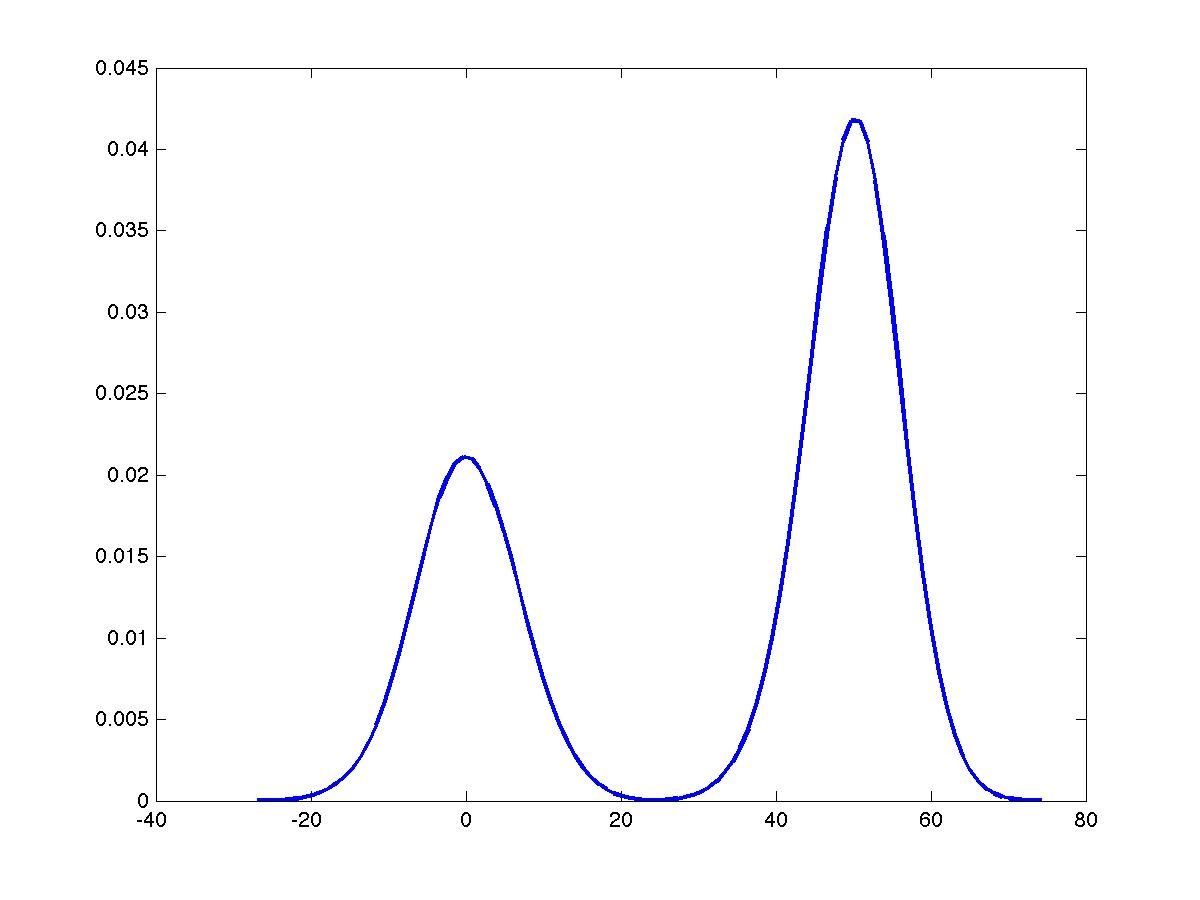
\includegraphics[width=0.5\textwidth]{bimodal.jpg}
	\caption{A sample bimodal distribution with two different modes.}
\end{figure}

It is interesting to note that as the number of vertex modes or categories for a graph goes from $2$ to $\infty$, the degree distribution among all vertices in the graphs, along with the hierarchy of peers in the graph, will begin to resemble that of a scale-free graph. Therefore, one can think of bimodal graphs as a special case of scale-free graphs that are useful when the power-law nature of the degree distribution complicates analytical efforts.

\section{Network Robustness Optimization Methods}

The standard robustness optimization method used in literature has been the application of large-scale stochastic simulations (usually in the form of Monte Carlo simulations) that perform robustness calculations for random graphs after individual links or nodes are removed from the network. As such, the problem of finding network topologies that yield optimal values for robustness are translated into mixed-integer nonlinear optimization problems that attempt to maximize the number of nodes or links that must be removed from the network in order for it to become globally disconnected. In this section, we discuss a sample of such efforts and the results that were found.

\begin{comment}
\subsection{Random and Scale-Free Graph Investigations}

Following the insight that hostile vertex attacks that target important nodes with large degrees tend to cause the most significant damage to a network, Albert et al. performed extensive studies on the robustness of random and scale-free graphs. By examining each of these classes of graphs in the context of random vertex deletions and targeted vertex attacks, it has been shown that random graphs are more robust against intentional vertex attacks, whereas the scale-free graphs are more robust against random deletions. This can be seen in Figure \ref{RandomResults}, where the breaking point of the largest component of the graphs $S$ drops off quicker for random graphs when attacked randomly \cite{GraphThesis}.

\begin{figure}[ht]
	\label{fig:RandomResults}
	\centering
		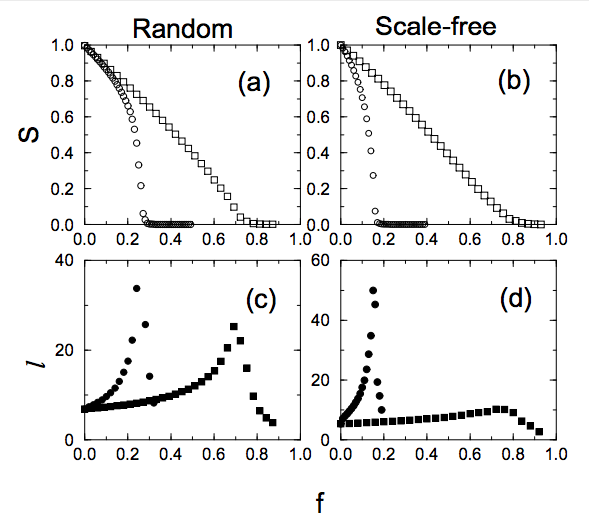
\includegraphics[width=0.5\textwidth]{random_results.png}
	\caption{Results of the random and scale-free graphs varied as $f$, the fraction of nodes removed from each graph, is changed.} %\cite{GraphThesis}
\end{figure}
\end{comment}

\subsection{Fractional Node Deletion Investigations} 
Paul et al studied the robustness of random graphs in the context of random node deletions \cite{Paul}. Their work was driven by simulations that approximated the fraction of nodes $f_c$ that would need to be removed from random networks in order for the graph to become globally disconnected. Formally, $f_c$ can be defined in terms of the number of "hub" nodes$q$ that must be removed. In order to find the optimal value for $q$, a Monte Carlo search was performed over a large set of random graphs that were structured according to a special degree distribution that assumes each network consisted of $q$ hub nodes and $N - q$ leaf nodes. The search algorithm utilized during these simulations was shown in Algorithm \ref{alg1}. 

\begin{algorithm}
\caption{Monte Carlo $q$ Search}
\label{alg1}
\begin{algorithmic}
	\item 1. Initialize a graph $G$ with $N$ vertices.
	\item 2. Randomly delete a node in the network and calculate $\kappa(G)$.
	\item 3. Increment $q$ by 1 node.
	\item 4. If $\kappa < 2$, $G$ has become disconnected, so terminate and return $q$. Otherwise, decrement $q$ by 1 and go to step 2.
\end{algorithmic}
\end{algorithm}

The resulting fraction of ndoes that needed to be deleted is $f_c = \langle n_r \rangle / N$, which is referred to as the fractional threshold. This threshold was then compared against $q$ to determine the robustness of graphs in terms of the number of hub nodes. This is natural because the hub nodes provide more backup routines for traffic in the event of random failures in the network. It was determined that the optimal value of $q$ that maximizes the network robustness is as follows:
\begin{eqnarray}
q = \left[(\langle k \rangle - 1) / \sqrt{\langle k \rangle}\right]\sqrt{N},
\end{eqnarray}
where each of these vertices have degree $\sqrt{\langle k \rangle N}$. Thus, for a graph $G = (V,E)$ with $N$ vertices, $q$ "hubs" would need to be removed in order to make $G$ disconnected, and thus $f_c = q/N$.
Paul et al also examined the the relationship between $q$, $f_c$, and $N$, as shown in Figure 3. In essence, they were able to conclude that the number of $hub$ nodes needed to achieve optimal robustness increased logarithmically with the increase in $N$. This result implies a network construction heuristic that assumes the number of hubs should be logarithmically proportional to the size of a network. 

\begin{figure}[h!]
	\label{fractionalResults}
	\centering
		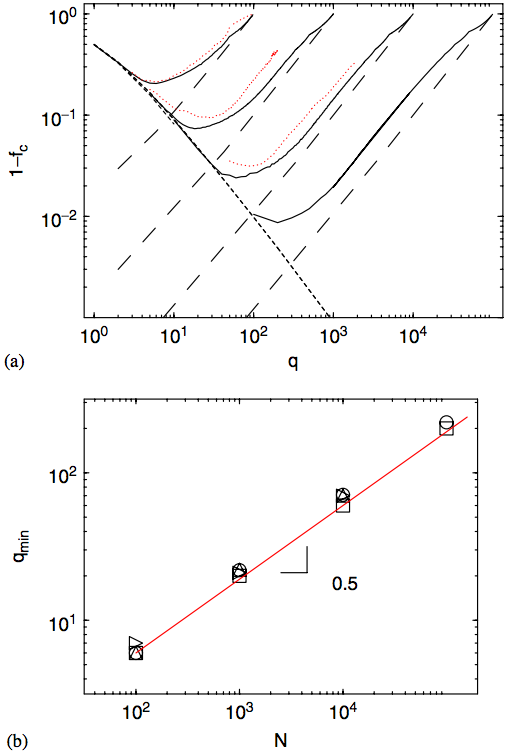
\includegraphics[width=0.5\textwidth]{fractional_results.png}
	\caption{Figure $a$ shows that as the number of hub nodes increases in a network of $N$ nodes, the fraction of nodes that needs to be deleted increases (since the value $1 - f_c$ decreases). Figure $b$ shows that the number of hubs $q$ increases logarithmically with the number of nodes in a network of $N$ nodes.}
\end{figure}

%TODO: read http://polymer.bu.edu/hes/articles/pshs06.pdf and discuss the metric here - devote entire section to it in the NR part

\subsection{Fixed-Degree Distribution Investigations}

Independent to the work done by Paul et al, Herrmann et al also conducted research on optimization algorithms that increase this robustness measure while at the same time maintaining the distribution of vertex degrees throughout the network. Their proposed algorithm seeks to re-arrange node edges and connections to improve the resilience of the host network to any kinds of attacks using Monte-Carlo simulations. This algorithm can be described as follows:
\begin{algorithm}
\caption{Robustness Optimization}
\label{alg2}
\begin{algorithmic}
	\item 1. Choose two random edges $(a,b)$ and $(c,d)$ from the graph $G$.
	\item 2. Replace these edges with $(a,c)$ and $(b,d)$.
	\item 3. If $R_{new} > R_{old}$, accept the swap and go to step 1. Otherwise, revert the swap and goto step 1. 
\end{algorithmic}
\end{algorithm}
Algorithm~\ref{alg2} is repeated for a very large number of iterations until an ideal level of robustness has been obtained, albiet at the sake of sometimes massive computations (as is the case with Monte-Carlo methods).
An interesting result from their optimization efforts was that every graph structure seemed to converge towards an onion-like toplogy, meaning that there are distinct layers of nodes that are connected, and that each layer $i$ has more connectivity than its parent layer $i+1$ \cite{Onion}. Another interesting property of the onion graph is that for almost every pair of vertices $u, v \in V(G)$ with the same degree, there exists a a path between $u$ and $v$ that does not contain any vertex of a higher degree, which is an indication that the degree distribution closely resembles a bimodal distribution. An example of such a graph with $124$ nodes and $366$ edges is shown in Figure 4.

\begin{figure}[h!]
	\label{fig:Onion}
	\centering
		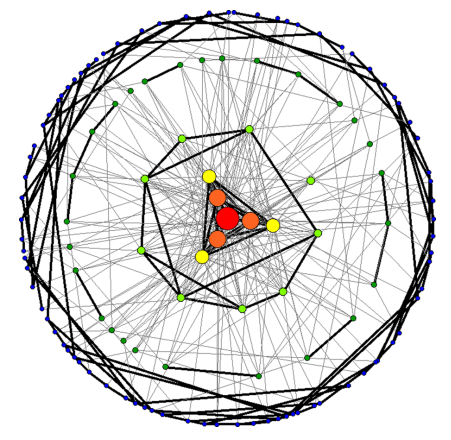
\includegraphics[width=0.5\textwidth]{Onion.jpg}
	\caption{An example of a graph with $124$ nodes and $366$ edges that exhibits the onion-like topology.} %\cite{Onion}
\end{figure}

%%%%%%%%%% Bimodal discussion, how they simulated and concluded that bimodal was the best

\section{Evolutionary Network Construction}
%http://www.springerlink.com/content/3621163544501342/?MUD=MP
One more recent investigation of graphs with fixed degree distributions was performed by Sonawane et al \cite{bimodal}. However, their approach was unique in that instead of starting with a random graph on $N$ vertices, they start with a graph on $0$ vertices and then iteratively build an optimally robust network by considering 

As shown in the previous section, networks with bimodal degree distributions tend to have high measures of robustness against targeted attacks and random failures. While it is possible to perform optimization on an existing graph of $N$ vertices to obtain such graph topologies (as was done in the work by Herrmann et al), such initial network knowledge is not known or cannot be assumed. Therefore, various methods to construct networks with bimodal degree distributions have been proposed to address this issue. 

One recent evolutionary method developed by Sonawane et al iteratively constructs a network with a bimodal degree distribution by adding nodes and links to the network with probability $p$ and then removing arbitrary links with probability $(1-p)$ at each iteration. Their approach has been empirically verified to generate graphs with bimodal degree distributions with Monte Carlo simulations that run up to $10,000$ iterations (i.e. generate networks with $10,000$ nodes).  A high-level pseudocode description of the evolution procedure is shown in Algorithm 3.

\begin{algorithm}
\caption{Bimodal Network Evolutionary Generation}
\label{alg2}
\begin{algorithmic}
	\item 1. Let $G = (\emptyset, \emptyset)$. 
	\item 2. Create a new vertex $v_1$ and add it to $G$
	\item 3. Iteratively create new vertices $v_i$ and add them to $G$ with probability $p$ and link them to other vertices $v_j \in V(G)$ with probability $1-p$. Repeat until the desired iteration count has been reached.
\end{algorithmic}
\end{algorithm}

In order to further test the correctness of this method the authors varied the construction probability $p$ used in the algorithm. Their simulation results concluded that the resulting degree distribution was minimally effected by the variation in $p$. Lower order networks showed the most impact by varying $p$, as indicated in Figure 5. In order to revive the bimodal degree distribution it is necessary to evolve the network using the same algorithm to a larger number of vertices, because the size of the network corresponds to its correlation with the bimodal degree distribution when constructed in this manner \cite{bimodal}.

\begin{figure}[h!]
	\label{fig:distribution}
	\centering
		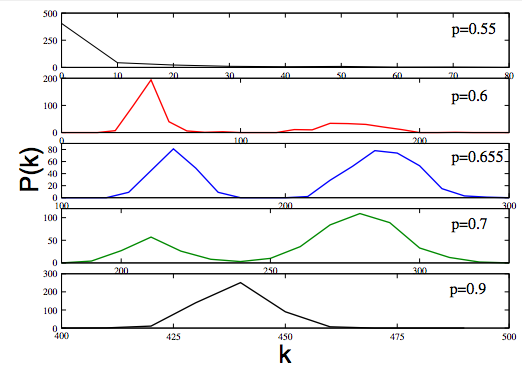
\includegraphics[width=0.5\textwidth]{evol_distribution.png}
	\caption{The degree distribution $P(k)$ for a network of $500$ vertices with average degree $k$ by varying $p$ over the set of values $\{0.55, 0.6, 0.655, 0.7, 0.9\}$. Notice that the inner three values for $p$ resulted in the most bimodal distribution, while the remaining values tended towards other distributions.}
\end{figure}

\section{Conclusion}
Network robustness is a very important issue that must be considered with designing and constructing mission-critical networks of every scale that are susceptible to targeted attacks or random failures. The robustness of every network is highly influenced by its underlying topology. Furthermore, those with the most optimal measures of robustness tend to resemble the onion-like structure or are characterized by having scale-free or bimodal degree distributions. Current research trends will surely continue to reveal more information about the relationship between the network toplogy and its measure of robustness, and this information must be utilized in order to make networks resistent to any kind of failure. 

\bibliography{nr}

\end{document}
